% !TeX spellcheck = it_IT
\section{Control Flow Integrity CFI}
\label{sec:cfi}

Si tratta di una tecnica di protezione basata su un'idea diversa dalle altre difese descritte precedentemente, le quali "complicavano" l'attacco prevenendone le fasi. 

Qua il paradigma di difesa è diverso, si vuole una cosa più generale, l'idea è quella di \textbf{definire un modello di comportamento del programma} e se l'esecuzione effettiva esce da questo modello viene segnalata un'anomalia.

Le "sfide" di questa idea sono: 
\begin{itemize}
	\item definire il modello di comportamento, qual'è il comportamento aspettato
	
    \item rilevare efficientemente e velocemente deviazioni dalle aspettative
	
    \item evitare possibili compromissioni del detector/monitor che controlla il programma
\end{itemize}

\paragraph{Definire expected behavior:} Come si può \textbf{caratterizzare il comportamento di un programma} durante l'esecuzione? Una caratteristica fondamentale di tutti i programmi è il control flow, rappresentabile tramite \textbf{Control Flow Graph CFG}, in cui ogni nodo è una chiamata a funzione (insiemi di istruzioni) e gli archi sono i passaggi di stato del programma. 

Il CFG rappresenta il flusso del programma in termini di insiemi di istruzioni e transizioni tra di essi. Se durante l'esecuzione effettiva il comportamento non rispetta le transizione definite: anomalia.

\paragraph{Rilevare deviazioni efficientemente:} Il controllo deve essere rapido, quindi il monitor deve essere efficiente. Non può essere esterno perché diventerebbe troppo invasivo. Il controllo viene quindi inserito all'interno del programma: \textbf{In-line reference monitor IRM}: istruzioni di controllo inserite all'interno del programma stesso. 

I controlli vanno fatti rispetto a un \textbf{threat model} ben definito: si suppone quali siano le possibili azioni che l'attaccante può o non può compiere e i controlli vengono inseriti di conseguenza. 

Ad esempio: si presuppone che l'attaccante 
\begin{itemize}
	\item può fare stack e heap overflow, ROP
    
	\item non può disabilitare l'IRM, non può modificare il codice in memoria (DEP)
\end{itemize}

Va sempre definito un threat model con ciò che è e non è lecito fare da parte dell'attaccante. Se l'attaccante riesce a rompere questi presupposti il sistema di difesa viene effettivamente superato (ad esempio, disabilita l'IRM saltando i check).

\paragraph{Evitare compromissione del detector:} Per evitare che l'IRM venga disabilitato sicuramente serve che il codice sia immutabile e che sia presente una sufficiente randomness all'intero dei controlli stessi. 

L'in-line monitor deve essere protetto da immutabilità e randomness.

In termini di \textbf{efficienza}: il \textbf{Classic CFI} (2005 di Microsoft Research) portava un overhead medio del 16\%, con 45\% nel caso peggiore; funzionava solo su eseguibile, non sulle librerie. Nel 2014 si è raggiunto il \href{https://www.cse.psu.edu/~gxt29/papers/mcfi.pdf}{\textbf{\texttt{Modular CFI}}} (\href{https://www.cse.psu.edu/~gxt29/}{\texttt{pagina autore}}), un modello di CFI modulare con un overhead molto più basso (5\% in media, 12\% worst case), il quale è in grado di lavorare anche su librerie.

\paragraph{Sicurezza:} MCFI permette di ridurre del 95.75\% i gadget ROP; definendo punti di entrata e uscita dell'esecuzione non si può portare avanti un attacco ROP, il quale, per definizione, modifica il flusso del programma; MCFI blocca i salti illeciti. 

La percentuale di riduzione viene dal fatto che i gadget non possono essere utilizzati in quanto non parte del flusso di controllo originale, significativamente riducendo la superficie di attacco. Si possono usare solo i gadget presenti all'interno del flusso di esecuzione (pochi).

Un'altra metrica usata è l'\textbf{Average Indirect-target Reduction (AIR)}, ovvero la percentuale di riduzione di possibili bersagli di salti indiretti che un attacco potrebbe sfruttare (punti di controllo del control flow). Le istruzioni di salto possono essere categorizzate in 
\begin{itemize}
	\item \textbf{direct calls}: viene definito esplicitamente l'indirizzo a cui saltare (direct, salta a quell'indirizzo)
    
	\item \textbf{indirect calls}: tutte le operazioni in cui l'indirizzo finale del salto va calcolato a runtime
\end{itemize}
In sostanza, la percentuale di bersagli per salti indiretti che vengono eliminati dalla CFI, ovvero quasi tutti.

\subsection{Costruzione del Control Flow}

La costruzione del control flow di un programma è divisa in due fasi: 
\begin{itemize}
	\item analisi statica
    
	\item analisi dinamica
\end{itemize}

\paragraph{Analisi statica:} Il compiler costruisce il grafo del control flow (già presente, viene usato per ottimizzazione, "strumenta" il programma). 

Il primo passo dell'analisi statica è il \textbf{call graph}, ovvero il grafo che rappresenta le chiamate a funzione; quale funzione chiama cosa. Esempio: 

\begin{center}
	\begin{minipage}[h]{0.52\textwidth}
		\begin{minted}{java}
sort2(int a[], int b[], int len)
{
    sort(a, len, lt);
    sort(b, len, gt);
}
		\end{minted}
	\end{minipage}
    \hfill 
	\begin{minipage}[h]{0.37\textwidth}
		\begin{minted}{java}
bool lt(int x, int y) {
    return x<y;
}
bool gt(int x, int y) {
    return x>y;
}
		\end{minted}
	\end{minipage}
\end{center}

\begin{center}
	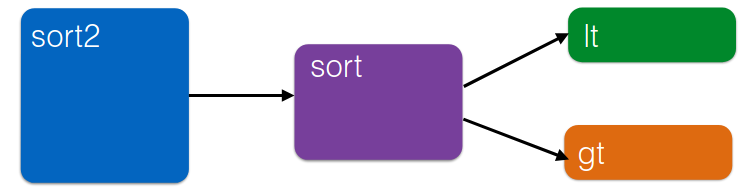
\includegraphics[width=0.8\linewidth]{img/cfi/call1}
\end{center}

Permette di rappresentare il \textbf{flusso di chiamate} all'interno del control flow, ma si tratta di un modello piuttosto permissivo: rappresenta le chiamate ma non il flusso reale delle funzioni.

Idealmente si vorrebbe un modello \textit{più restrittivo}, ovvero \textbf{il CFG}; si introducono i \textbf{basic blocks}: contenitori di istruzioni sequenziali, terminate da un'istruzione di salto, di qualsiasi tipo (\texttt{jmp}, \texttt{ret}, \texttt{\dots}). Permette di distinguere \texttt{call} da \texttt{return}, il grafo sul codice di prima diventa:
\begin{center}
	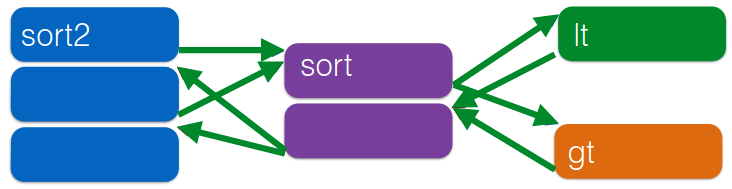
\includegraphics[width=0.8\linewidth]{img/cfi/call2}
\end{center}

Ogni funzione viene "spezzata" in moduli, ognuna delle quali ha una \texttt{call}/\texttt{return}, definendo meglio il modello di esecuzione del programma. Ogni basic block fa una \texttt{call} o una \texttt{return} (praticamente un gadget). 

In sostanza:
\begin{itemize}
	\item viene calcolato il CFG di \texttt{call}/\texttt{return} a compile time (o comunque partendo dal binario)

	\item il control flow del programma viene monitorato dall'interno, assicurando che segua percorsi definiti dal CFG

	\item le direct calls non vanno monitorate (assumendo che il codice sia immutabile, l'indirizzo target non può essere cambiato), quindi \textbf{solo le indirect calls vanno controllate} (\texttt{jmp}, \texttt{call}, \texttt{ret} con target non costanti, tutti i salti parametrici)
\end{itemize}

\subsection{In-Line Monitor}

Bisogna implementare all'interno del programma un metodo efficace per controllare "da dove arriva" un salto, inoltre deve essere una "trasformazione" del programma. 

Per fare ciò vengono usate delle \textbf{label}:
\begin{itemize}
	\item viene inserita come commento una label all'inizio del basic block destinazione del salto, riga non di codice

	\item prima di saltare, viene fatta una \texttt{cmp} tra il valore presente nella destinazione (dove punta il registro su cui viene fatto il salto) e il valore che dovrebbe avere la label

	\item se coincidono tutto a posto, manda avanti l'esecuzione

	\item se non coincidono blocca il programma
\end{itemize}

\newpage % Inevitabile, sorry Tino

Il codice
\begin{table}[h!]
	\centering
	\begin{adjustbox}{max width=\textwidth}
	\begin{tabular}{@{} lll | lll @{}}
		\multicolumn{3}{c}{\bfseries Source} & \multicolumn{3}{c}{\bfseries Destination} \\
		\cmidrule(lr){1-3} \cmidrule(l){4-6}
		\bfseries Opcode bytes & \bfseries Instructions &
		& \bfseries Opcode bytes & \bfseries Instructions & \\
		\midrule
		\texttt{FF E1} & \texttt{jmp ecx} & \texttt{; computed jump}
		& \texttt{8B 44 24 04} & \texttt{mov eax, [esp+4]} & \texttt{; dst} \\
		\multicolumn{6}{c}{\dots} \\
	\end{tabular}
	\end{adjustbox}
\end{table}

Diventa:

\begin{table}[h!]
	\centering
	\begin{adjustbox}{max width=\textwidth}
	\begin{tabular}{@{} lll | lll @{}}
		\multicolumn{3}{c}{\bfseries Source} & \multicolumn{3}{c}{\bfseries Destination} \\
		\cmidrule(lr){1-3} \cmidrule(l){4-6}
		\bfseries Opcode bytes & \bfseries Instructions &
		& \bfseries Opcode bytes & \bfseries Instructions &\\
		\midrule
		\texttt{81 39 78 56 34 12}
		& \texttt{cmp [ecx],\,12345678h} & \texttt{; comp ID \& dst}
		& \texttt{78 56 34 12} & \texttt{data 12345678h} & \texttt{; ID} \\
		\texttt{75 13}
		& \texttt{jne \_error\_label} & \texttt{; if \(\neq\) fail}
		& \texttt{8B 44 24 04} & \texttt{mov eax, [esp+4]} & \texttt{; dst} \\
		\texttt{8D 49 04}
		& \texttt{lea ecx,[ecx+4]} & \texttt{; skip ID at dst}
		& \multicolumn{3}{c}{\dots} \\
		\texttt{FF E1}
		& \texttt{jmp ecx} & \texttt{; jump to dst}
		& & & \\
	\end{tabular}
	\end{adjustbox}
\end{table}

Viene inserita \textbf{una label per ogni basic block}, quando c'è un indirect call il programma controlla che la destinazione abbia la label corretta (o una delle label corrette) prima di saltare. Viene controllato che il salto sia alla destinazione corretta.

\paragraph{Tipi di labeling:} Il \textbf{labeling} può essere: 
\begin{itemize}
	\item \textbf{semplice}: una stessa label per tutti i blocchi; evita chiamate fuori dal grafo ma non impedisce salti errati; permette "quello che vuoi" all'interno del grafo
    
	\item \textbf{dettagliato}: una label diversa a seconda dei punti di ritorno, permettendo di controllare anche che i salti all'interno del grafo siano corretti
\end{itemize}

\paragraph{Can we defeat CFI?}
\begin{itemize}
	\item Code injection con label corretti: non si può fare perché i dati non sono eseguibili (DEP)
	
    \item Modificare label nel codice per permettere il control flow desiderato: il codice è immutabile
	
    \item Modificare lo stack durante il check per controllarne l'esito: l'attaccante non può modificare i registri in cui sono caricati i dati rilevanti al controllo (No time-of-check, time-of-use bug TOCTOU)
\end{itemize} 

\paragraph{Garanzie:} Il CFI garantisce di impedire attacchi che modificano il control flow (ROP, ret2libc, \dots). Ma non 
\begin{itemize}
	\item attacchi che manipolano il control flow seguendo le label (mimicry attacks, soprattutto con labeling semplice)

	\item data leaks: \href{https://www.heartbleed.com/}{\texttt{Heartbleed}} non sarebbe stato bloccato

	\item corruptions: modificare variabili di controllo per portare al flusso di esecuzione desiderato (e.g, overflow di una variabile "\texttt{authenticated}" su cui viene fatto un controllo)
\end{itemize}